\subsection{Procedimentos Experimentais}
\label{subsec:proc_exp}

A execução da rota escolhida — saponificação a quente da mistura de óleos — foi realizada em bancada conforme descrito nesta seção, já incorporando as adaptações apresentadas anteriormente. Para cada amostra produzida, foram separados os seguintes materiais:

\begin{itemize}
    \item becker de 600~ml de vidro (para os óleos);
    \item becker de 100~ml de plástico (para a pesagem do NaOH);
    \item becker de 100~ml de vidro (para a solução de NaOH em água);
    \item proveta de 50~ml;
    \item balança analítica;
    \item aquecedor;
    \item agitador mecânico;
    \item suporte de metal (para fixação do agitador);
    \item 2 muflas;
    \item termômetro;
    \item 1 garra;
    \item bastão de vidro.
\end{itemize}

\noindent Reagentes:

\begin{itemize}
    \item óleo de coco babaçu;
    \item óleo de soja;
    \item ácido esteárico;
    \item etanol;
    \item NaOH;
    \item água.
\end{itemize}

O arranjo dos materiais na bancada é apresentado na Figura~\ref{fig:arranjo_material}, e o processo pode ser resumido pelo fluxograma da Figura~\ref{fig:fluxograma_sabao}.

\begin{figure}[H]
    \centering
    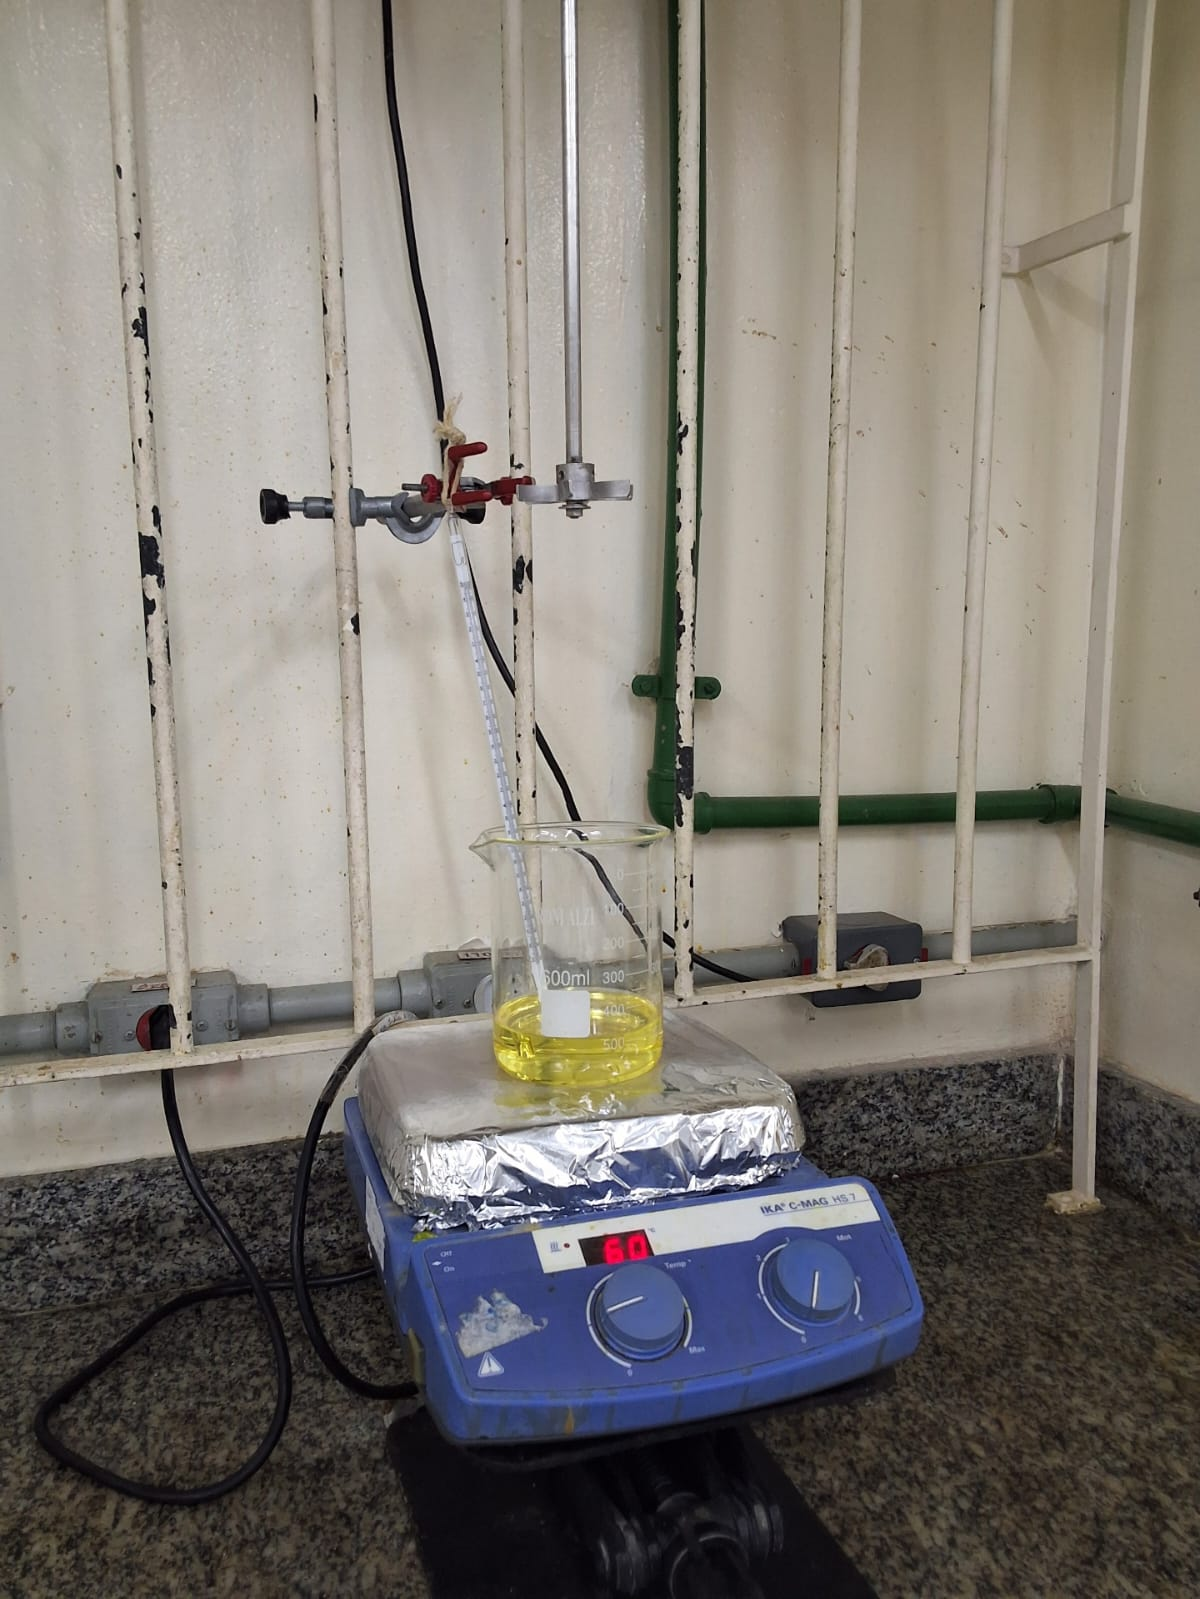
\includegraphics[width=0.4\textwidth]{src/fig/preparativos/arranjo_materiais.jpg}
    \caption{Arranjo dos materiais na bancada \newline (agitador deveria estar em contato do óleo).}
    \label{fig:arranjo_material}
\end{figure}

\begin{figure}[H]
    \centering
    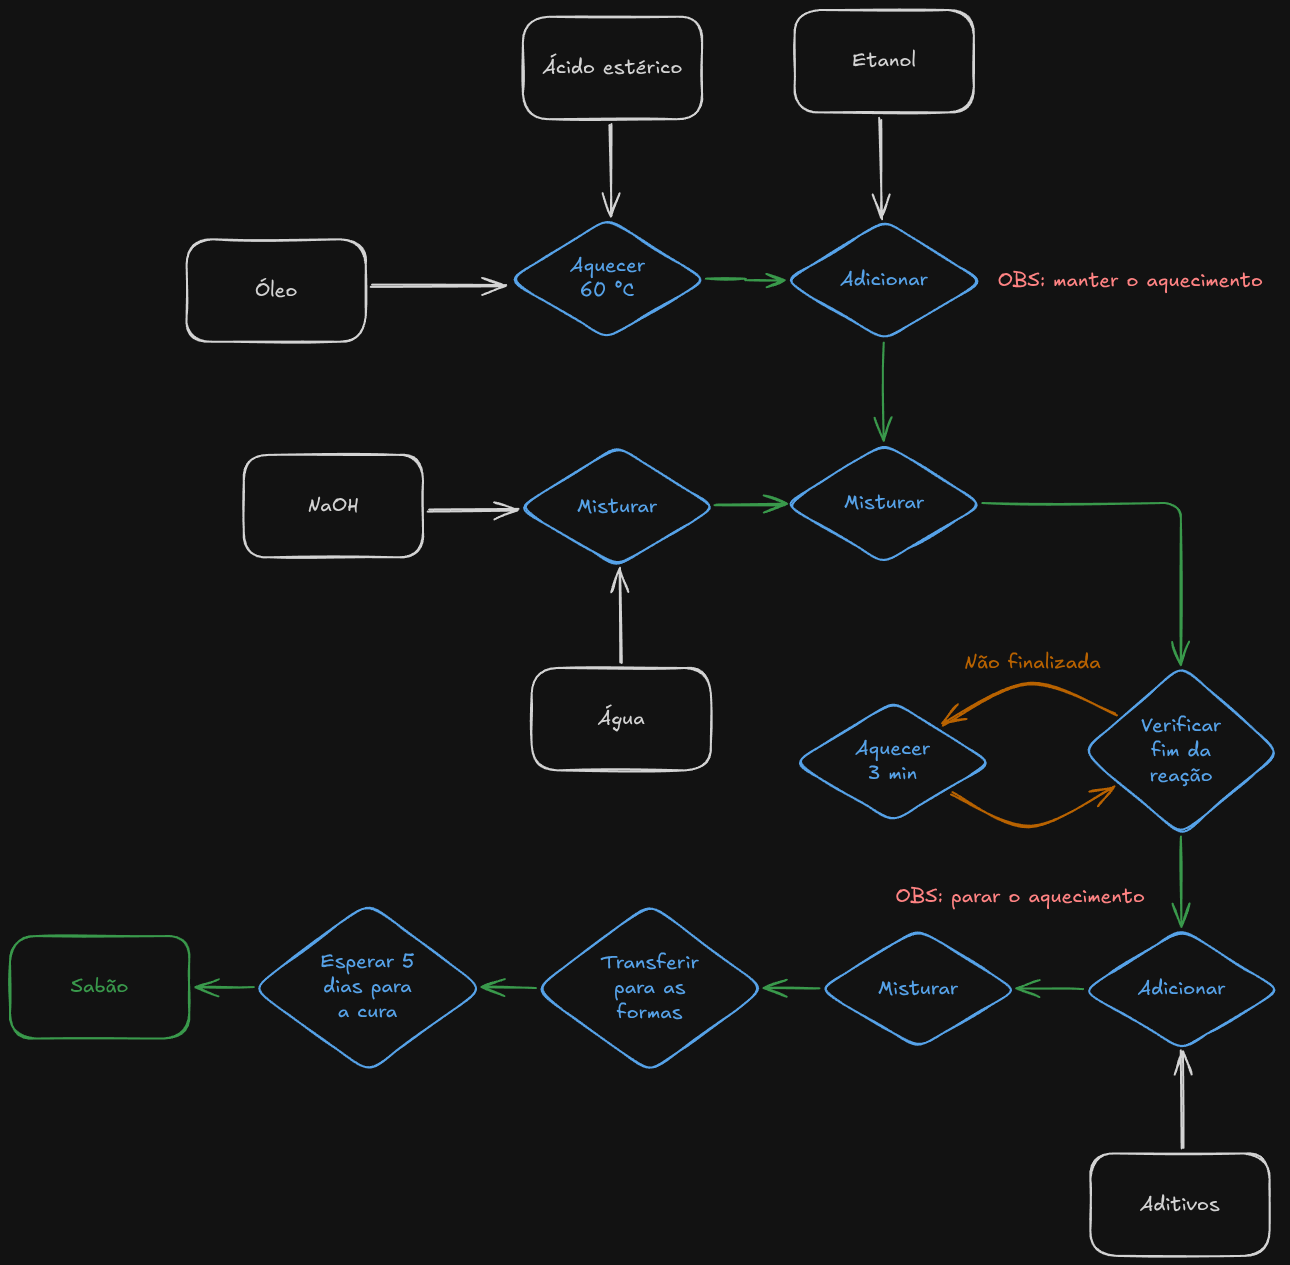
\includegraphics[width=0.9\textwidth]{src/fig/preparativos/fluxograma_sabao.png}
    \caption{Fluxograma do processo de produção do sabão.}
    \label{fig:fluxograma_sabao}
\end{figure}

\subsubsection{Preparação inicial do óleo}

Inicialmente, prepara-se a mistura de óleos totalizando 120~g em um becker de 600~ml, medindo-se a massa de cada óleo com o auxílio da balança. Para a produção de sabão não são necessárias medidas exatas, sendo válidos valores aproximados. Caso a amostra utilize ácido esteárico, este deve ser adicionado junto aos óleos nesta etapa, conforme a Figura~\ref{fig:prepara_oleo}. Para agilizar a dissolução do ácido esteárico na mistura de óleos recomenda-se aquecer a mistura para valores acima de 70~°C e inferiores a 120~°C.

\begin{figure}[H]
    \centering
    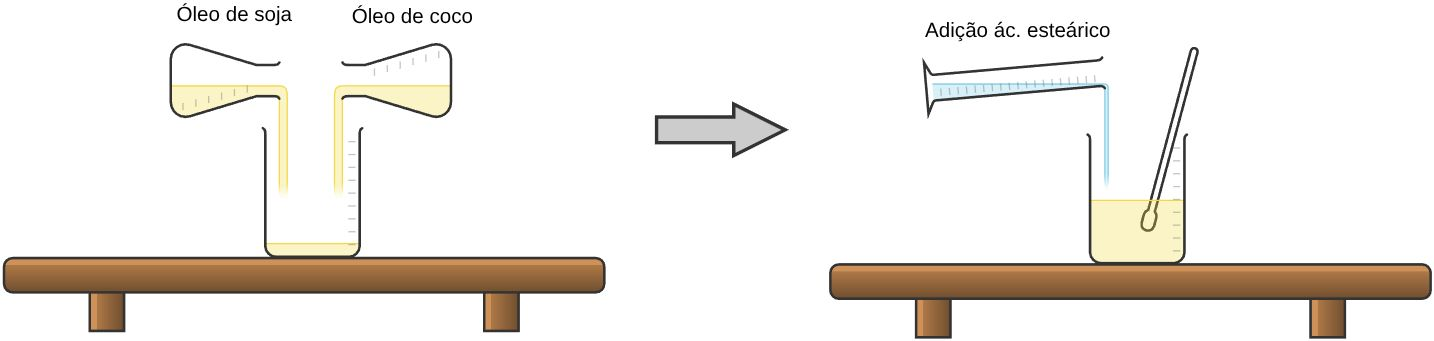
\includegraphics[width=0.8\textwidth]{src/fig/preparativos/prepara_inicial_oleo.jpg}
    \caption{Preparação inicial da mistura de óleos.}
    \label{fig:prepara_oleo}
\end{figure}

Em seguida, a mistura é levada ao aquecimento até 60~°C. Durante o aquecimento do óleo, deve-se iniciar a preparação da solução alcalina (Figura~\ref{fig:oleos_60}).

\begin{figure}[H]
    \centering
    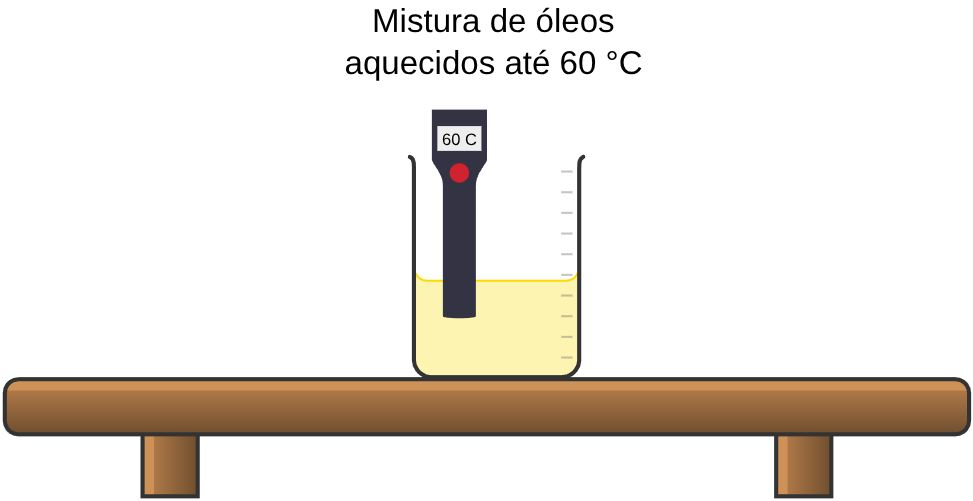
\includegraphics[width=0.4\textwidth]{src/fig/preparativos/oleos_60.jpg}
    \caption{Mistura de óleos aquecida a 60~°C.}
    \label{fig:oleos_60}
\end{figure}

\subsubsection{Preparação inicial da solução alcalina}

Durante esta etapa, deve-se prestar muita atenção à temperatura do óleo, sendo ideal que uma pessoa fique responsável por mantê-la na faixa adequada. Como o NaOH disponível no laboratório é sólido, a preparação da solução básica é bastante simples. Primeiro, utilizando luvas, pesa-se a quantidade de NaOH necessária para a amostra, empregando o becker de plástico (ou um de vidro, se disponível).

Após a pesagem, preenche-se um becker de vidro com água destilada. A quantidade de água segue a regra de 25\% da massa de óleo, em mililitros; assim, para amostras de 120~g, utilizam-se 30~ml de água. Com os materiais prontos, na capela, dissolve-se o NaOH na água — é fundamental que a \textbf{base seja adicionada à água}, e não o contrário, e que isso ocorra aos poucos. Ao final, a solução deve estar transparente; caso ainda apresente aspecto opaco, a base não está totalmente dissolvida (Figura~\ref{fig:solucao_naoh}).

\begin{figure}[H]
    \centering
    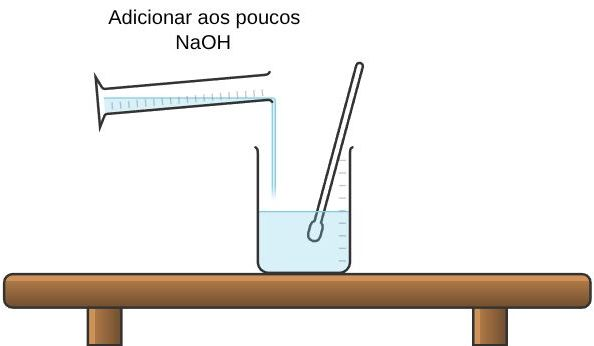
\includegraphics[width=0.4\textwidth]{src/fig/preparativos/solucao_NaOH.jpg}
    \caption{Solução alcalina de NaOH.}
    \label{fig:solucao_naoh}
\end{figure}

\subsubsection{Cálculo da quantidade de álcool}
\label{subsubsec:calc_alcool}

Quando o etanol é empregado como cossolvente, o procedimento prevê o uso de etanol a 50\% em um volume equivalente a uma fração do volume da mistura de óleos, que pode variar entre 5\% e 20\% conforme o ajuste desejado. Como o etanol disponível no laboratório possui concentração de 95\%, é necessário convertê-lo de modo a manter a mesma quantidade de etanol puro. Igualando a quantidade de etanol puro nas duas concentrações, obtém-se a Equação~\ref{eq:alcool}.

\begin{equation}
    0,95 \cdot V_{95\%} = 0,50 \cdot V_{50\%}
    \label{eq:alcool}
\end{equation}

\noindent em que $V_{50\%}$ é o volume previsto pelo procedimento, igual à fração escolhida do volume de óleo ($V_{50\%} = f \cdot V_{\text{óleo}}$, com $f$ entre 5\% e 20\%). Isolando o volume de etanol a 95\%, chega-se à Equação~\ref{eq:alcool_isolado}.

\begin{equation}
    V_{95\%} = \frac{0,50}{0,95} \cdot f \cdot V_{\text{óleo}}
    \label{eq:alcool_isolado}
\end{equation}

\subsubsection{Mistura das soluções}

Caso a amostra utilize etanol, este deve ser adicionado ao óleo imediatamente antes da adição da solução básica (Figura~\ref{fig:adicao_etanol}).

\begin{figure}[H]
    \centering
    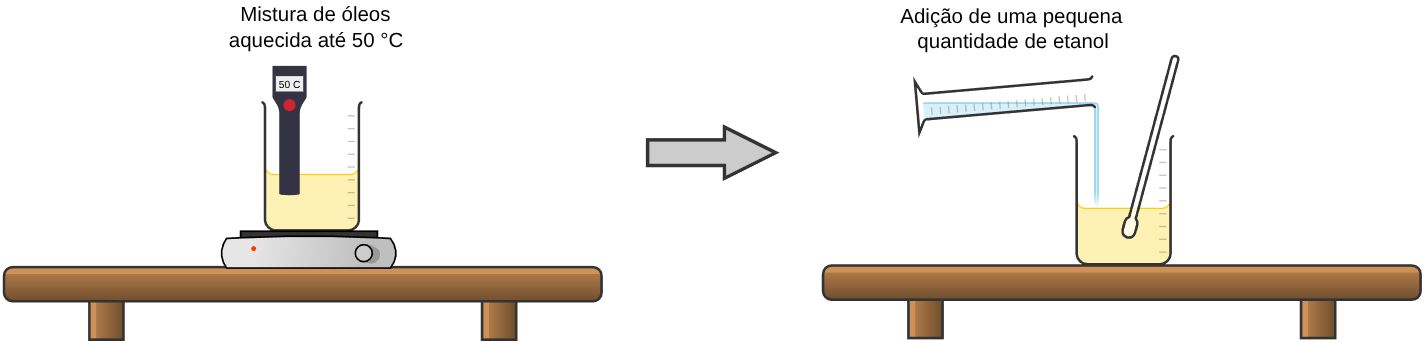
\includegraphics[width=0.8\textwidth]{src/fig/preparativos/adicao_etanol.jpg}
    \caption{Adição de etanol ao meio oleoso.}
    \label{fig:adicao_etanol}
\end{figure}

A solução alcalina é então adicionada ao becker maior, de 600~ml, que contém o óleo. Em seguida, inicia-se uma agitação vigorosa, mantendo-se o aquecimento a 60~°C durante todo o processo (Figura~\ref{fig:mistura_solucoes}).

\begin{figure}[H]
    \centering
    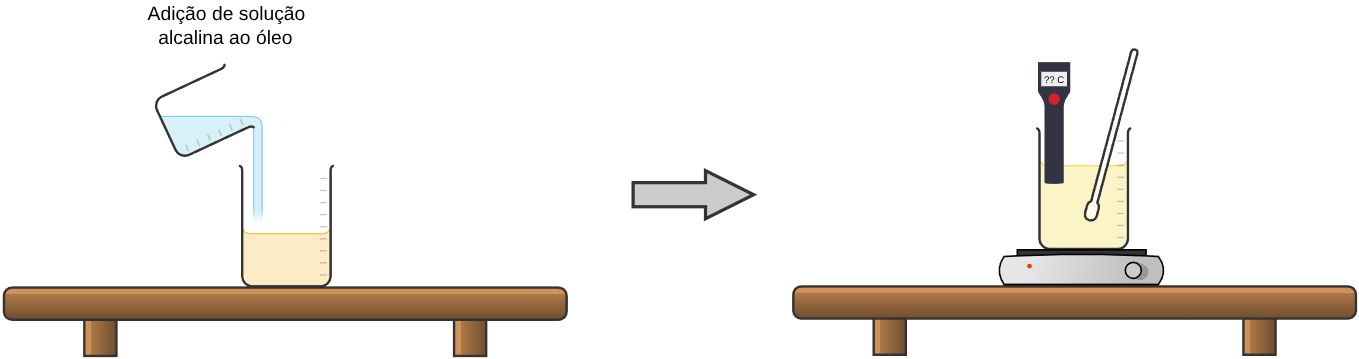
\includegraphics[width=0.8\textwidth]{src/fig/preparativos/mistura_solucoes.jpg}
    \caption{Mistura das soluções oleosa e alcalina.}
    \label{fig:mistura_solucoes}
\end{figure}

\subsubsection{Validação do fim da reação}

Decorridos cerca de 15 minutos do início da mistura, espera-se que a reação já esteja em estado adequado para a transferência do material aos moldes. Como isso nem sempre ocorre, nesses casos o produto deve ser avaliado a cada 3 minutos. A validação é feita tanto pela medição do pH quanto pela consistência do produto:

\begin{itemize}
    \item o pH deve estar na faixa entre 11 e 13;
    \item o produto deve apresentar consistência pastosa e homogênea, semelhante a um purê de batatas.
\end{itemize}

Ao final da etapa de bancada, o produto é colocado em moldes para iniciar o processo de cura. Em média, para esse tipo de processo, de 3 a 5 dias são suficientes para a cura, de modo que 7 dias (uma semana) representam um período mais do que adequado.